\documentclass[11pt, titlepage]{article}
\usepackage{amsmath,amsthm,amssymb}
\usepackage{hyperref, pgf, tikz}
\usepackage{fancyhdr}
\usetikzlibrary{arrows}
\usepackage[margin=1.25in]{geometry}
\usepackage{graphicx}                     
\pagestyle{fancy}
\usepackage{array}
%\usepackage{wrapfig}

\lhead{Lab \#5}
\rhead{\thepage}
\cfoot{}

\title{Torques, Equilibrium, and Center of Gravity\\ \ \\ \large Lab \#5}
\author{Name: Avery Karlin \\ Partner: Nicholas Yang}
\date{}
\begin{document}

\maketitle

\begin{center}
\LARGE Torques, Equilibrium, and Center of Gravity
\end{center}

\section*{Objective}
The objective of the lab is to measure the spring constant of springs, and the spring constant when they are in series, parallel, and on opposite sides.

\section*{Introduction}
The period of an oscillation is defined as the time for one full cycle of oscillation, while the frequency is defined as the number of cycles per second, such that $f = \frac{1}{T}$. Angular frequency is further defined as the number of radians per second, such that $\omega = 2\pi f$, defined on a spring oscillation as $\omega = \sqrt{\frac{k}{m}}$. As a result, we can use that to derive the formula $$k = \frac{4\pi^2m}{T^2}.$$

\section*{Procedures and Results}
%Procedure

\begin{figure}[p]
\centering
\hspace*{-10.5cm}
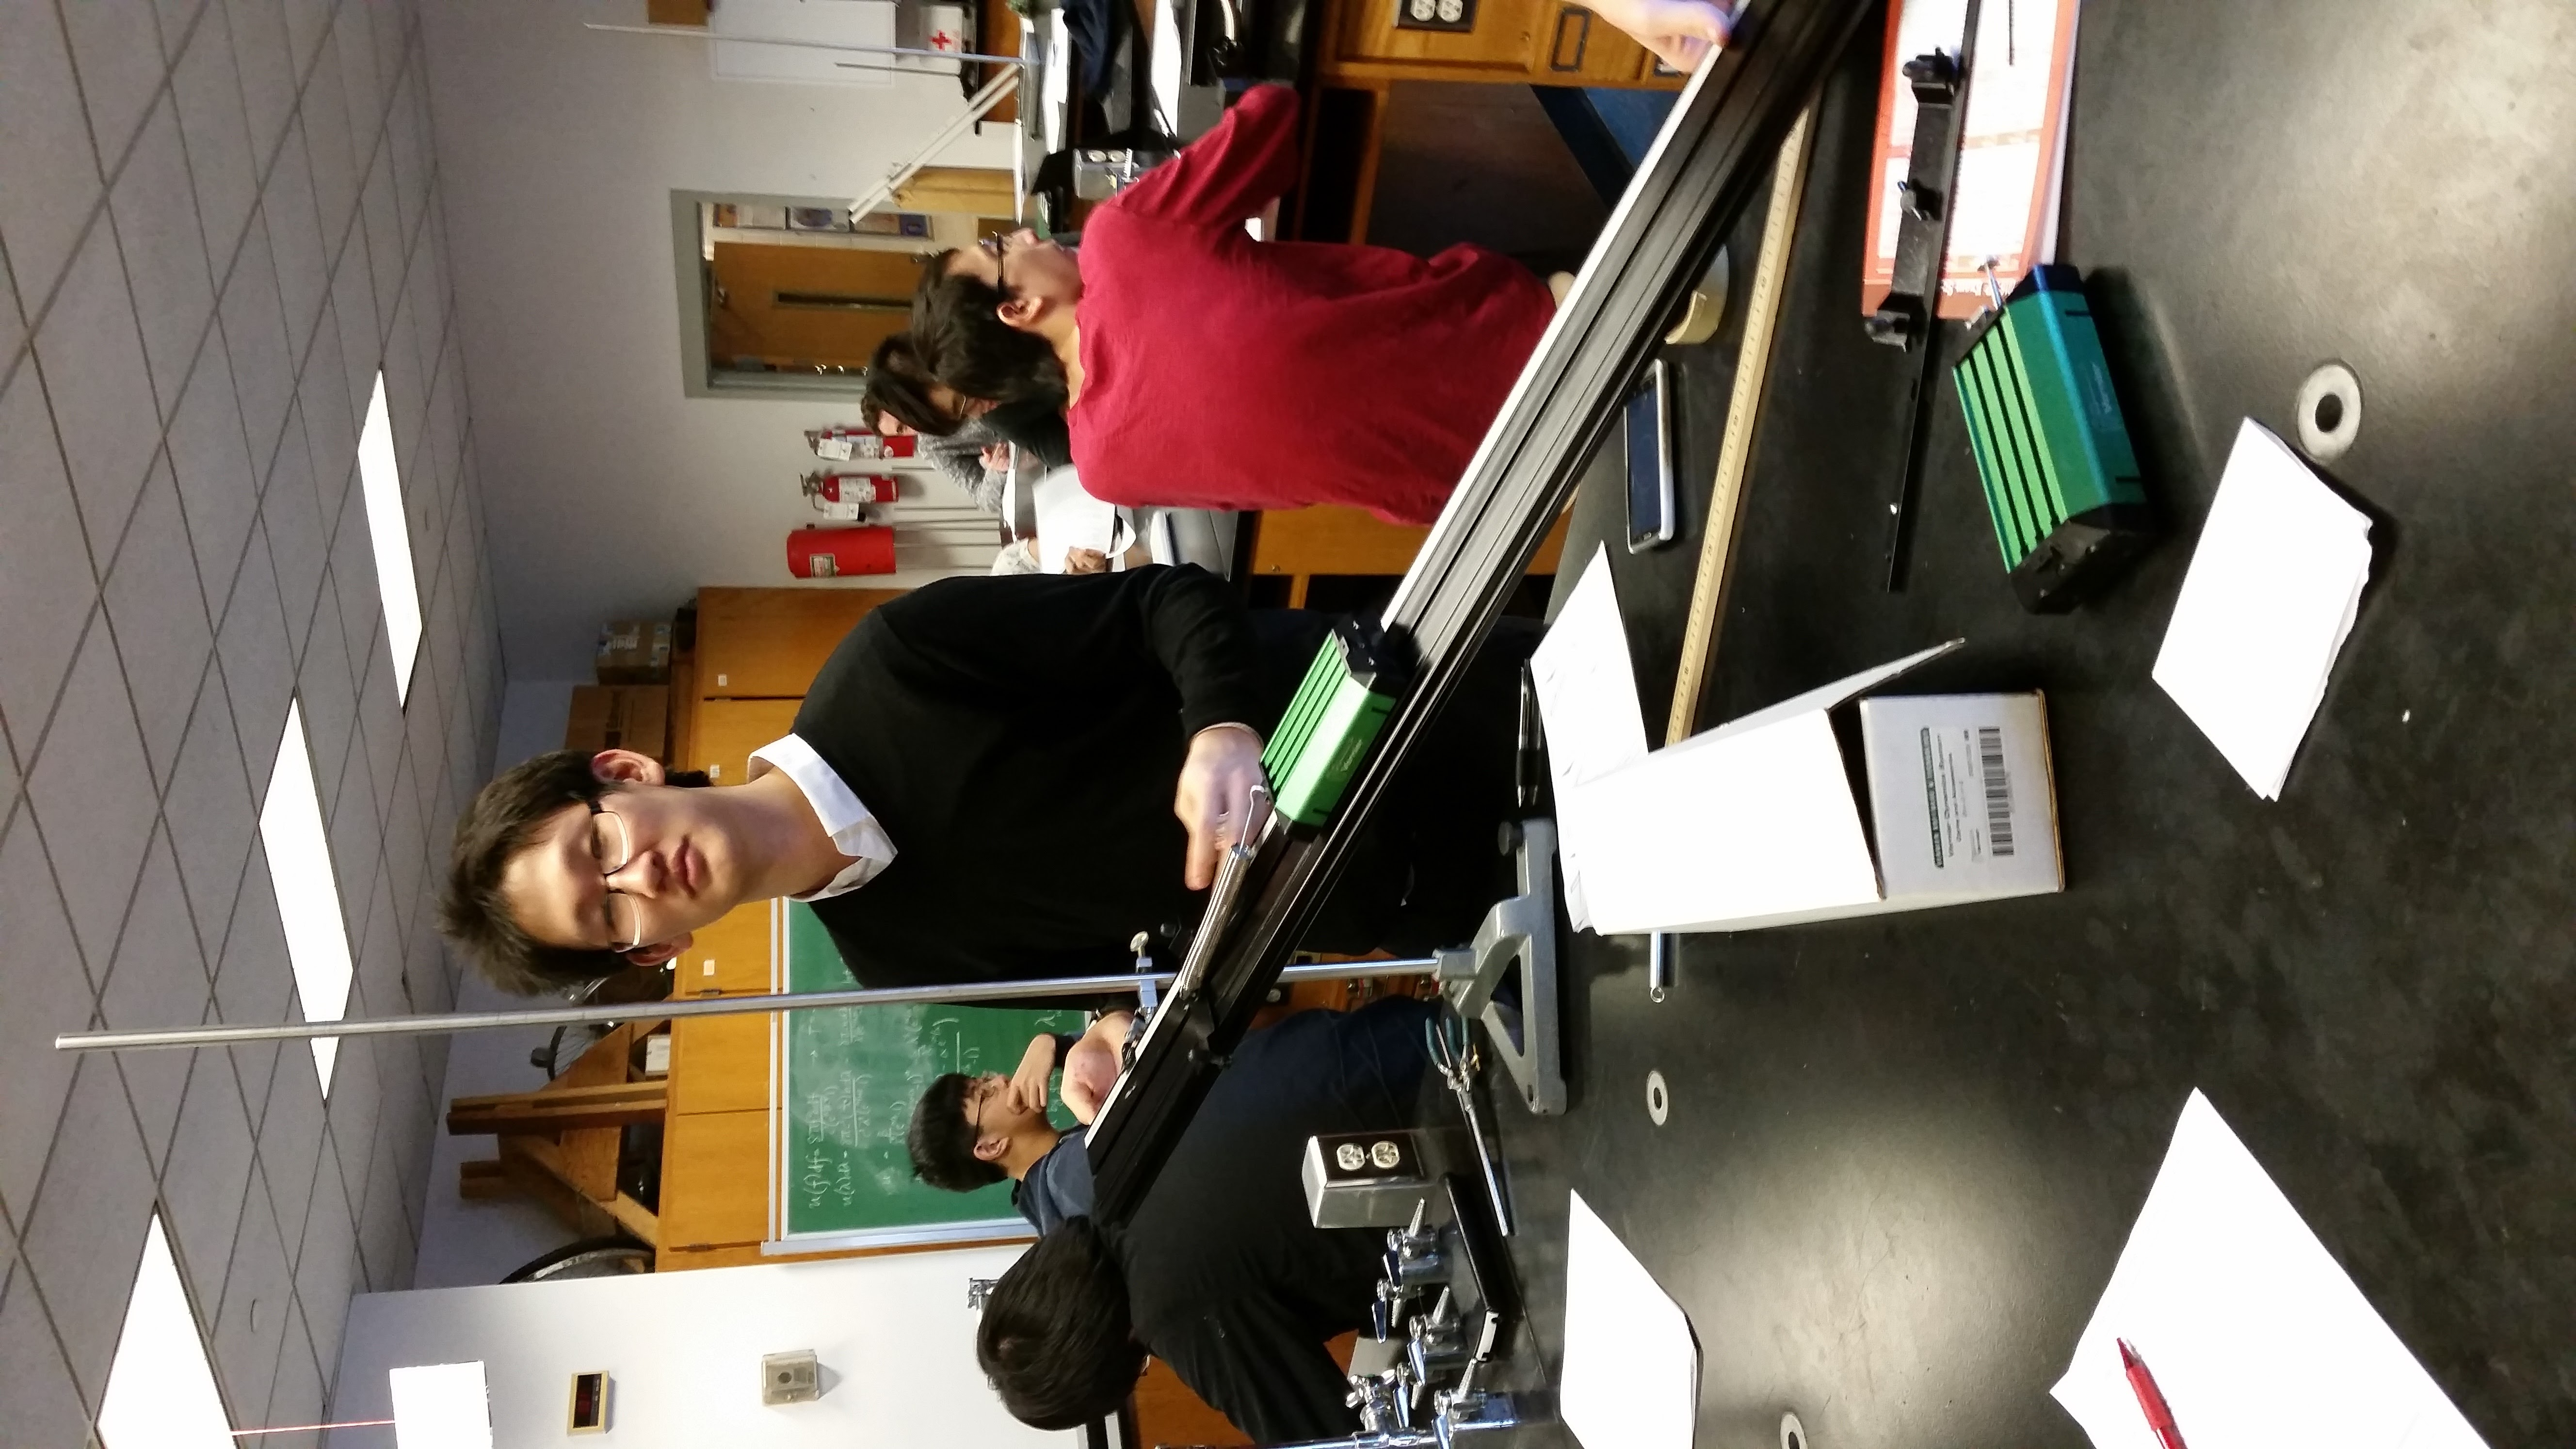
\includegraphics[scale=0.15, angle=270]{lab5.jpg}
\vspace*{19cm}
\end{figure}

\begin{center}
\begin{tabular}
{|m{5em}|m{5em}|m{5em}|m{5em}|m{5em}|m{5em}|}
Spring Format & Trial 1 (s) & 2 & 3 & 4 & 5 \\
Spring \#1 & 3.06 & 2.9 & 3.02 & 2.9 & 2.85 \\
Spring \#2 & 5.8 & 6.08 & 5.8 & 6.05 & 6.08 \\
Series & 6.75 & 6.73 & 6.53 & 6.46 & 6.77 \\
Parallel & 2.56 & 2.88 & 2.68 & 2.6 & 2.88 \\
Opposite & 2.7 & 2.78 & 2.68 & 2.83 & 2.65 \\
\end{tabular}
\end{center}

\section*{Discussion}
Sample calculations for the non-measured data are as shown:

$$k_t = k_1 + k_2 = 9.61 + 2.377 = 11.987 N*m$$
$$k_t = \frac{1}{\frac{1}{k_1} + \frac{1}{k_2}} = \frac{1}{\frac{1}{9.61} + \frac{1}{2.377}} = 1.906 N*m$$

$$\text{Series Percent Error} = \frac{|k_{act} - k_{exp}|}{k_{act}} * 100\% = \frac{|1.906 - 1.887|}{1.906} * 100\% = 0.996\% $$ 
$$\text{Parallel Percent Error} = 5.98\% $$
$$\text{Opposite Percent Error} = 6.53\% $$

\begin{center}
\begin{tabular}
{|m{8em}|m{8em}|m{8em}|m{8em}|}
Spring Format & Average (s) & Period (s) & k (N/m) \\\
Spring \#1 & 2.946 & 1.473 & 9.61 \\
Spring \#2 & 5.922 & 2.961 & 2.377 \\
Series & 6.648 & 3.324 & 1.887 \\
Parallel & 2.72 & 1.36 & 11.27 \\
Opposite & 2.728 & 1.364 & 11.204 \\
\end{tabular}
\end{center}

It is clear by the data that for springs in series, $\frac{1}{k_T} = \frac{1}{k_1} + \frac{1}{k_2}$, and for springs in parallel, $k_T = k_1 + k_2$. In addition, springs can be placed on opposite sides, where the overall $k_T = k_1 + k_2$, such that it acts as if it was in series.

The percent errors, especially that of the in series springs, are fairly low, such that the model used was correct. On the other hand, the error may have been the cause of not accounting for friction on the surface and drag for the cart on the surface. In addition, the high degree of precision in measuring the time could have introduced an element of human error. Finally, the springs themselves were not ideal, which could have made oscillation and the spring constant not fully consistant.

\section*{Conclusion}
It was found that in series springs have a spring constant of the reciprocal of the sum of the reciprocals of the individual spring constants, for a measured value of 1.887 N*m to the actual value of 1.906 N*m, for a percent error of 0.996\%.

Parallel springs have a spring constant of the sum of the individual spring constants, for a measured value of 11.27 N*m to the actual value of 11.987 N*m, for a percent error of 5.98\%.

Springs on opposite sides act as parallel springs for a spring constant of the sum of the individual spring constants, such that the measured value was 11.204 N*m to the actual value of 11.987 N*m for a percent error of 6.53\%.

\end{document}
